\section{Two Task Result}

First we consider the simplest case where there are only two tasks: one producing a value (task $A$) and one consuming it (task $B$). Considering just task $A$ we can see the worst case depicted in Figure~\ref{fig:2Tasks}. This scenario assumes schedulability to ensure that one job of $A$ must run and complete within each period. This is where our schedulability assumption becomes vital for our solution.

\begin{figure}[h]
	\centering
	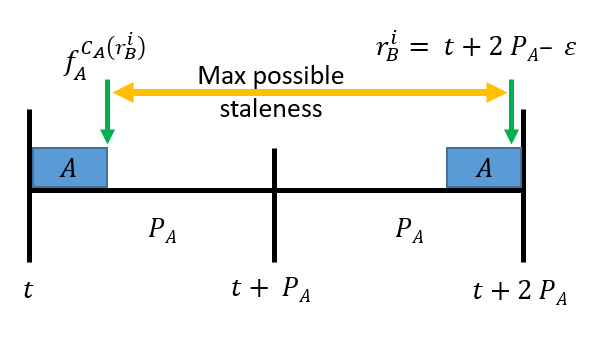
\includegraphics[width=0.3\textwidth]{figures/2TaskMaxStaleness}
	\caption{Maximum Staleness Scenario for Data from Task A.}
	\label{fig:2Tasks}
\end{figure}

Figure \ref{fig:2Tasks} labels the maximum separation between two publishes of output data from the depicted task. To maximize the staleness, we assume a job of task $B$ is released arbitrarily close to the finish of the second job of task $A$ and that the first (BCET) job of task $A$ ran to completion at the beginning of the previous period.

Note that we assume deadlines are equal to periods. However, it is easy to see here that a shorter deadline moves the latest possible execution of the second job of task A earlier, and hence decreases the max possible staleness. We will not consider this case further but it will be clear later how this could be substituted in place of our equal period and deadline example.

\begin{theorem}
	\label{thm:2TaskMaxWaiting}
	The scenario in Figure~\ref{fig:2Tasks} is the upper bound scenario for data freshness for data produced by a task.
\end{theorem}

\begin{proof}
	Note that one job must be executed within each period as per the definition of periodic tasks and our assumption of task set schedulability. Consider any placement of two jobs of a task within two consecutive periods. Assume this instance is not the one depicted in Figure~\ref{fig:2Tasks}. Then at least one of the following apply:
	\begin{case}
		The job in the first period is not completed as soon as possible. In this case, move the start of this job execution $\epsilon$ earlier. This increases the staleness by $\epsilon$.
	\end{case}
	\begin{case}
		The job in the second period is not completed as late as possible. In this case, move the start of this job execution $\epsilon$ later. This increases the staleness by $\epsilon$.
	\end{case}
	Since all other instantiations of the problem can be moved closer to the depicted instance while strictly increasing data staleness, it follows that the depicted instance is the unique worst case for output data staleness.
\end{proof}

Now that we have proven the above scenario is the worst case with regards to the freshness of data from task $A$, we can use algebra to solve for the constraint on $P_A$. From Figure~\ref{fig:2Tasks} we can see that the maximum staleness is composed of two periods of $A$ less one execution time of $A$ less $\epsilon$. We want this to be less than our freshness bound $d_{A \to B}$. We can then solve for $P_A$ to prove the following lemma.

Note that we assume the best case execution time and data delay for the first job in order to maximize staleness. The execution time of the second job is irrelevant.

\begin{lemma}
	\label{lem:2TaskResult}
	To ensure the output of task $A$ is always at most $d_{A \to B}$ old, choose $P_A \leq \frac{d_{A \to B} + E^{l,min}_A}{2}$.
\end{lemma}

\begin{proof}
	\begin{align*}
		d_{A \to B}&\geq 2P_A-E^{l,min}_A-\epsilon &\mbox{From Figure \ref{fig:2Tasks}}&\\
		P_A&\leq \frac{d_{A \to B} + E^{l,min}_A + \epsilon}{2} &\mbox{Rearrange}&\\
		P_A&\leq \frac{d_{A \to B} + E^{l,min}_A}{2} &\mbox{$\epsilon \to 0$}&
	\end{align*}
\end{proof}

We can justify bringing epsilon to zero as this is decreasing the period value and hence strictly increasing freshness. Thus if we set $P_A$ equal to the the above quantity we ensure that the output of task $A$ is always at most $d_{A \to B}$ old, and therefore can never be older when consumed by task $B$. We can also set $P_A$ less than this quantity and maintain the freshness guarantee.

Recall that our fitness metric is total utilization. It is trivial to see that choosing $P_A$ as large as possible will minimize the task set utilization. Thus the solution for the two task scenario while minimizing utilization is to set $P_A$ equal to the quantity in the lemma.
